\section{Results}
\label{sec:results}
\para{Aggregate performance.}
We analyze 1,935 rows with overall accuracy 0.835 and zero API error rows. The lower overall score is driven by harder tasks (\patterncls and \mgsmfr), not by numeral transduction.

\para{Core transduction findings.}
\Tabref{tab:core_band_results} shows near-ceiling results on \digitword and ceiling-level results on \worddigit. \gptfourone reaches 98.6\%--100\% on \digitword and 100\% in all \worddigit bands and conditions. \gptfouronemini direct remains high (96.7\%--100\% on \digitword; 100\% on \worddigit). These results do not support the predicted irregular-band degradation for transduction.

\begin{table*}[t]
\centering
\resizebox{\textwidth}{!}{%
\begin{tabular}{@{}llcccc@{}}
\toprule
Model & Condition & Task & 0--69 & 70--99 & 100--199 \\
\midrule
\gptfourone & Direct & \digitword & 0.9857 & {\bf 1.0000} & {\bf 1.0000} \\
\gptfourone & Reasoned & \digitword & 0.9857 & {\bf 1.0000} & {\bf 1.0000} \\
\gptfouronemini & Direct & \digitword & 0.9714 & 0.9667 & {\bf 1.0000} \\
\midrule
\gptfourone & Direct & \worddigit & {\bf 1.0000} & {\bf 1.0000} & {\bf 1.0000} \\
\gptfourone & Reasoned & \worddigit & {\bf 1.0000} & {\bf 1.0000} & {\bf 1.0000} \\
\gptfouronemini & Direct & \worddigit & {\bf 1.0000} & {\bf 1.0000} & {\bf 1.0000} \\
\bottomrule
\end{tabular}%
}
\caption{Band-wise transduction accuracy. Best values within each task block are in \textbf{bold}. \gptfouronemini reasoned was incomplete and is excluded.}
\label{tab:core_band_results}
\end{table*}


\para{Band-effect statistics.}
\Tabref{tab:significance_summary} summarizes irregular-vs-regular tests. For \digitword, neither \gptfourone direct ($+0.0059$, $p=0.6737$) nor \gptfouronemini direct ($-0.0216$, $p=0.3702$) is significant after FDR correction. In contrast, \patterncls shows large positive irregular-band effects in every complete run (all FDR-corrected $p<0.001$).

\begin{table}[t]
\centering
\resizebox{\linewidth}{!}{%
\begin{tabular}{@{}llrrr@{}}
\toprule
Model & Task & Risk diff. & $p$ & FDR sig. \\
\midrule
\gptfourone (direct) & \digitword & +0.0059 & 0.6737 & No \\
\gptfouronemini (direct) & \digitword & -0.0216 & 0.3702 & No \\
\gptfourone (direct) & \patterncls & +0.4353 & 5.29e-06 & Yes \\
\gptfourone (reasoned) & \patterncls & +0.4235 & 8.36e-06 & Yes \\
\gptfouronemini (direct) & \patterncls & +0.4805 & 1.58e-06 & Yes \\
\bottomrule
\end{tabular}%
}
\caption{Irregular-vs-regular band tests. Positive risk difference indicates higher accuracy on \irregularband.}
\label{tab:significance_summary}
\end{table}


\para{Pooled logistic regression.}
In the pooled core-probe model ($n=1775$), the irregular-band coefficient is positive and significant ($p\approx1.19\times10^{-9}$), while reasoned-vs-direct is not significant ($p\approx0.83$). This confirms that band effects exist in the combined probe space, but they are task-dependent rather than a uniform transduction failure.

\para{Prompt ablation on \mgsmfr.}
Reasoned prompting improves \gptfourone from 48.8\% to 57.5\% on \mgsmfr, an absolute gain of 8.75 points. This is substantially larger than condition effects in core transduction probes.

\begin{figure}[t]
    \centering
    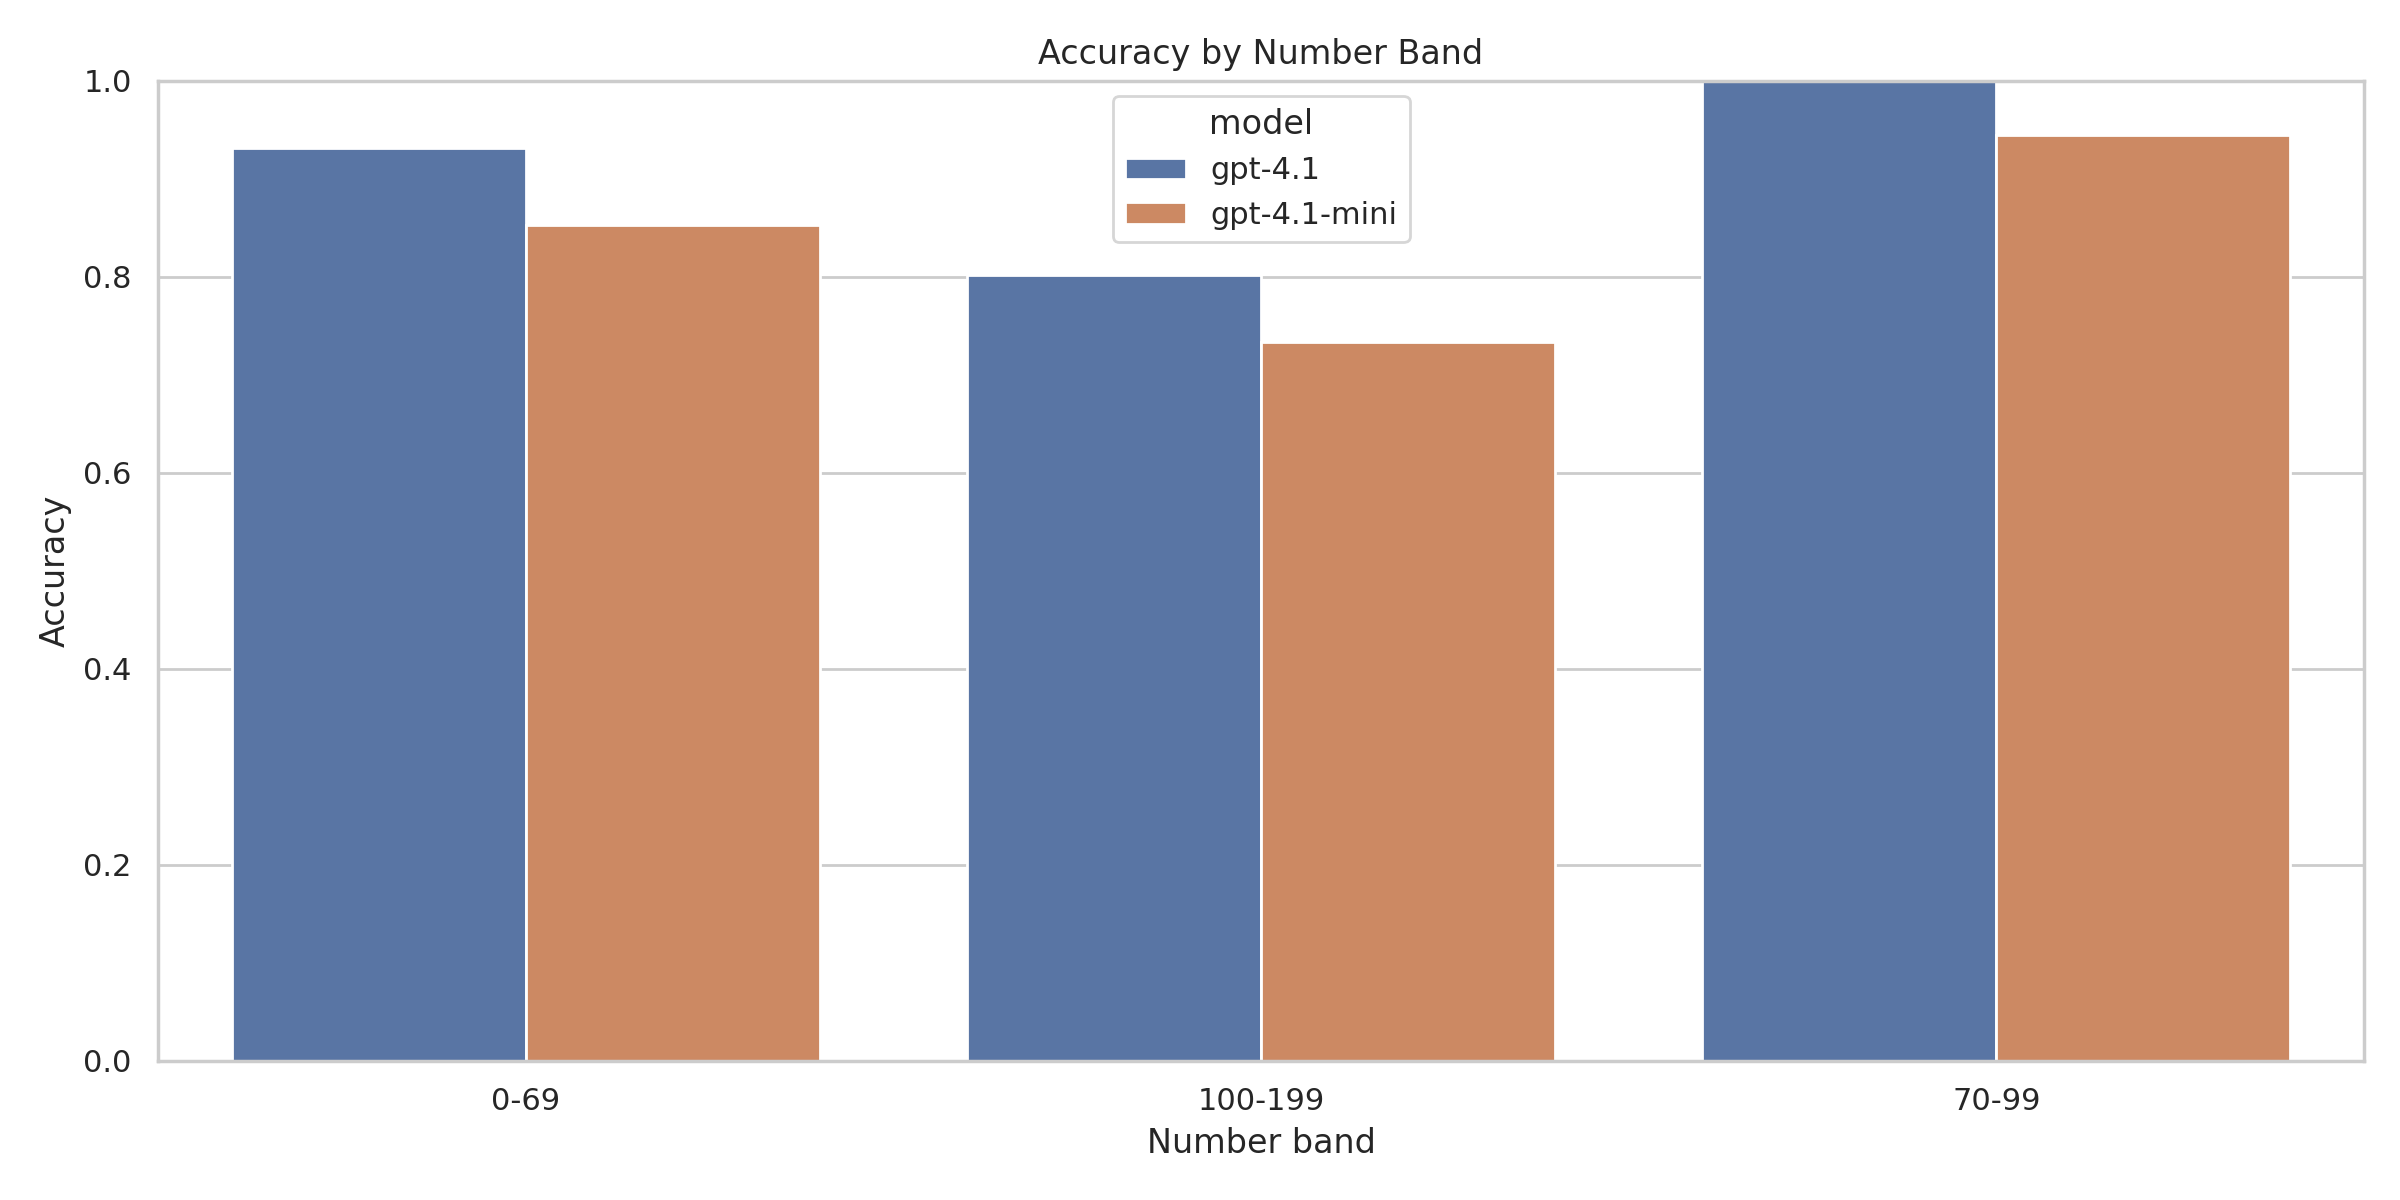
\includegraphics[width=0.95\linewidth]{figures/accuracy_by_band.png}
    \caption{Accuracy by number band, model, and task. Transduction tasks stay near ceiling, while \patterncls shows larger band separation.}
    \label{fig:accuracy_by_band}
\end{figure}

\begin{figure}[t]
    \centering
    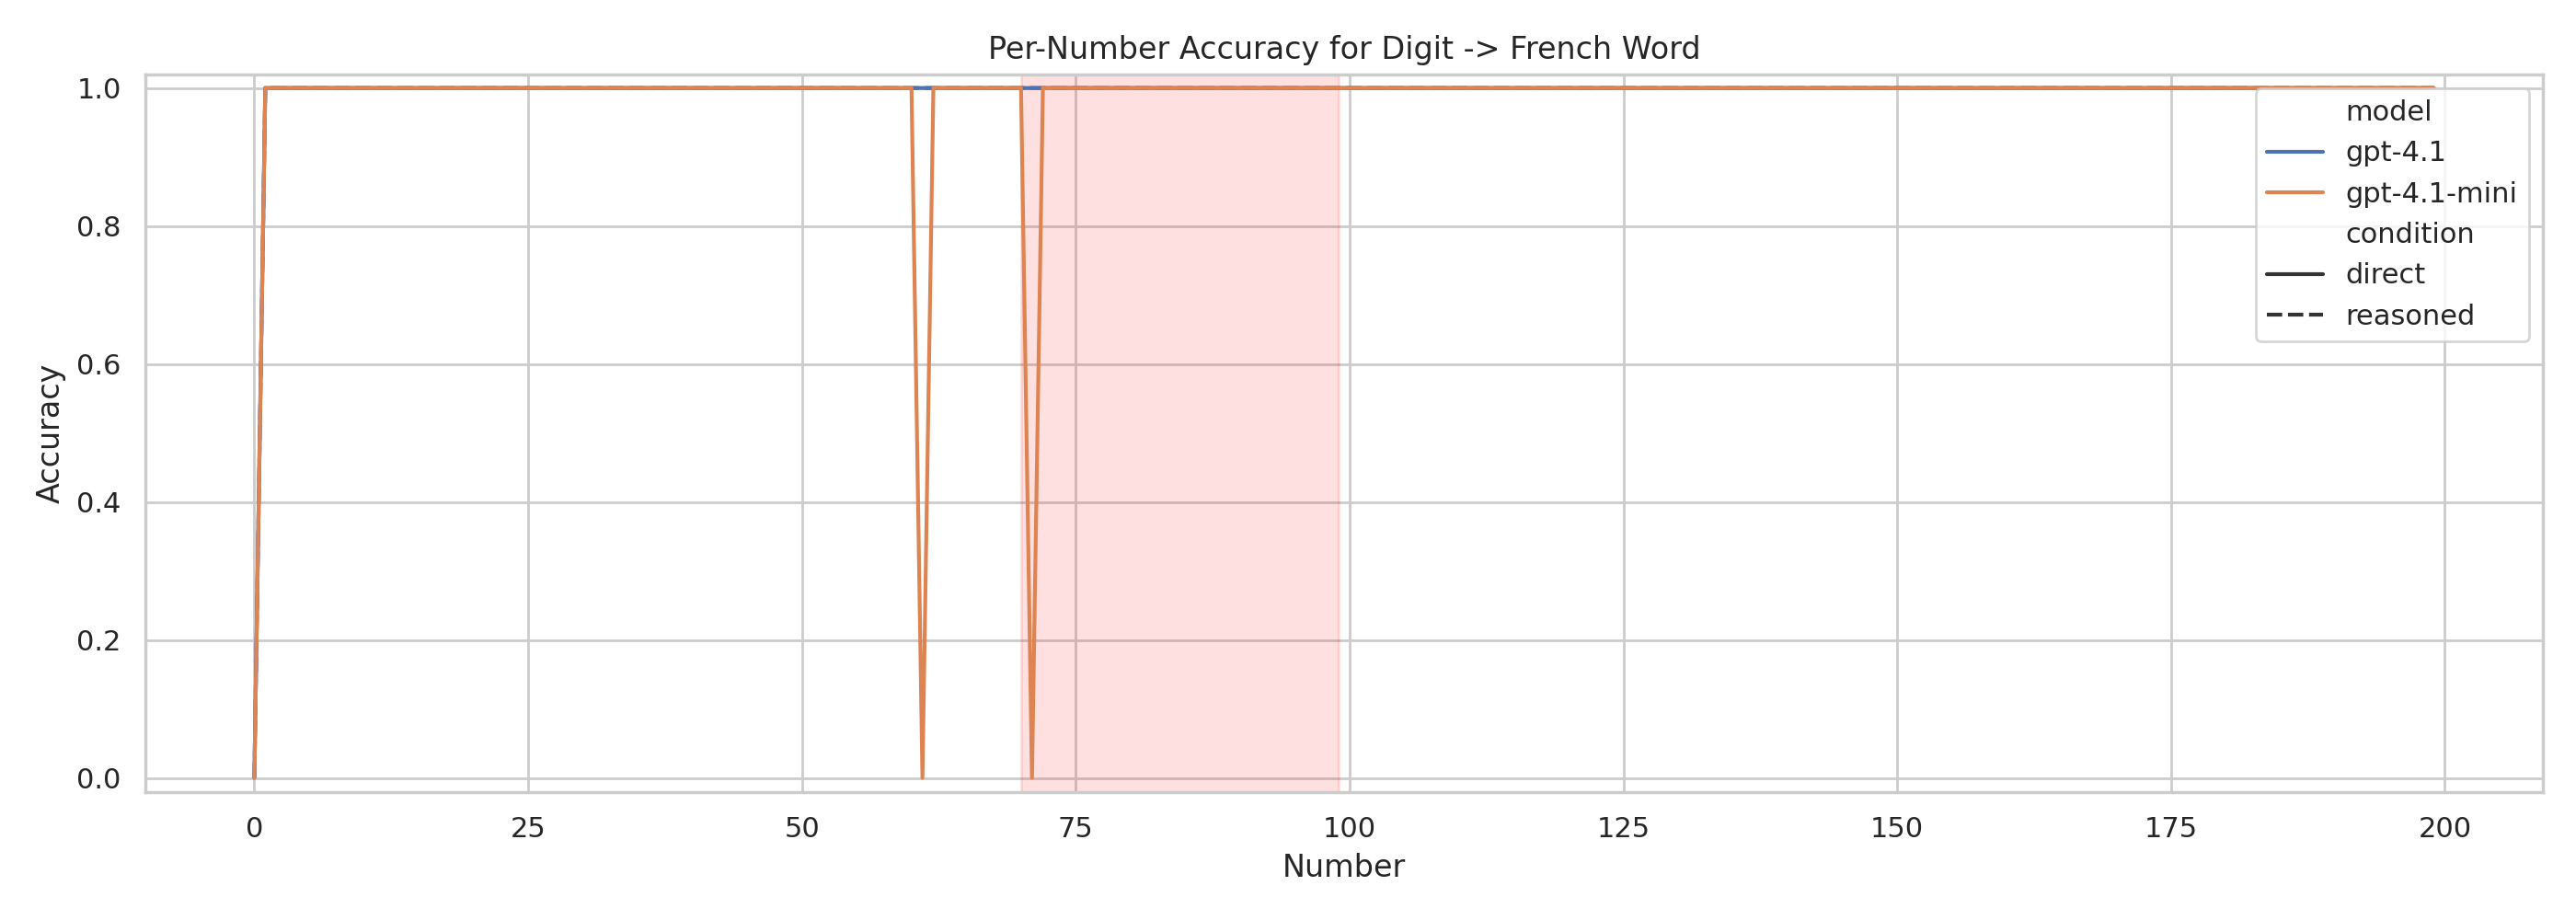
\includegraphics[width=0.95\linewidth]{figures/per_number_accuracy_digit_to_word.png}
    \caption{Per-number \digitword accuracy. Errors are sparse and not concentrated in the \irregularband range.}
    \label{fig:per_number}
\end{figure}

\para{Error analysis.}
Representative failures are mostly orthographic variants rather than numeric misunderstandings. For example, for 71 the model output \textit{soixante-et-onze} instead of canonical \textit{soixante et onze}; normalization resolves many such cases.
